\newpage
\section{Methodology}

\subsubsection{Design-Based Research}

Design-based research (DBR) is a research methodology aimed at improving educational practices through systematic, flexible, and iterative processes of analysis, design, development, implementation, and evaluation. It is grounded in collaboration between researchers and practitioners in real-world settings, ultimately producing design principles or theoretical contributions \parencite{wang_influence_2026}.

DBR is primarily conducted in authentic educational environments to bridge the gap between theoretical research and practical application \parencite{jong_design-based_2017}. Unlike traditional laboratory-based approaches, DBR is situated in naturalistic contexts where social interactions and environmental complexity are preserved and considered as integral parts of the research process \parencite{wang_influence_2026}.

A central feature of DBR is its iterative cycle, which consists of design, enactment, analysis, and redesign illustrated in \cref{fig:dbr_cycle}. The outputs of each cycle inform and guide subsequent cycles, enabling continuous refinement of both the intervention and the underlying theory \parencite{jong_design-based_2017}.


\begin{figure}[H]
\caption{Iterative cycle of Design-Based Research}\label{fig:dbr_cycle}
\centering
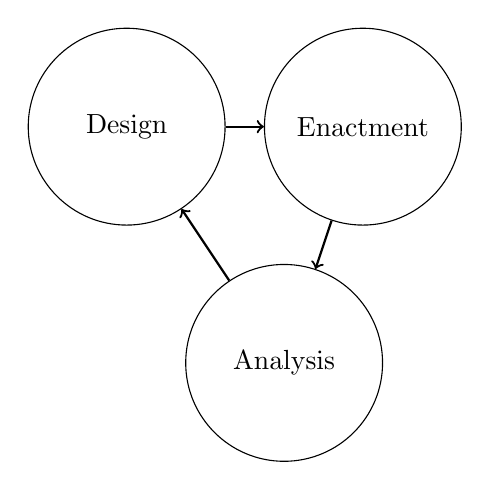
\begin{tikzpicture}[
    every node/.style={draw, circle, minimum size=2.5cm, align=center},
    arrow/.style={->, thick}
]

\node (design) at (0,0) {Design};
\node (enact) at (3,0) {Enactment};
\node (analysis) at (2,-3) {Analysis};

\draw[arrow] (design) -- (enact);
\draw[arrow] (enact) -- (analysis);
\draw[arrow] (analysis) -- (design);

\end{tikzpicture}
\end{figure}
\textcite{Beck2004XP} define Agile as a set of values and principles that emphasize iterative development, customer collaboration, and responsiveness to change. Agile development approaches typically include iterative and incremental development, self-organizing teams, and continuous feedback and adaptation.

Agile processes focus on the rapid and early delivery of working software and are based on development models that support incremental and iterative progress \parencite{keith2010agile}.

A user story is a description of a feature expressed from the perspective of the user and its intended value. User stories serve as the core unit of work in Agile development. Multiple user stories are maintained in a backlog, from which a subset is selected for implementation during a time-boxed iteration, typically lasting two to four weeks, known as a sprint. A collection of related user stories that collectively deliver a larger functional capability is referred to as an epic. Completed sets of functionality, such as alpha or beta versions, are commonly referred to as milestones.

User stories must be estimated, which requires sufficient understanding of both the system being built and the implementation approach. If the scope of a story is too large or insufficiently understood, accurate estimation becomes difficult. Such cases are often addressed through spikes, which are time-boxed research tasks used to reduce uncertainty \parencite{keith2010agile}.

Both DBR and Agile share a common iterative philosophy, in which development proceeds through cycles of analysis, implementation, evaluation, and refinement, enabling continuous learning and adaptation throughout the process.

% Object: Drone Physics

\subsection{Simulate the Quadcopter}

This section examines the flight dynamics and control implementation
found in the Yue's Ultimate Drone physics model \parencite{yuetility2022fpvphysics}. 

\subsubsection{Controller Mapping}

The flight controller distinguishes between unipolar throttle inputs and bipolar command sticks (Roll, Pitch, and Yaw): Throttle ($T$): Mapped to a normalized range of $[0, 1]$. Attitude Commands ($\theta, \phi, \psi$): Mapped to a range of $[-1, 1]$.

To refine the pilot's control over the aircraft, the system utilizes a non-linear control curve for joystick calculation. As \parencite{lovesay2003ergonomics} observes, a good quality force tracking controller has a linear output, with joystick force directly proportional to sight velocity, but many systems shape the joystick voltage output, to achieve fine control and greater tracking accuracy as the joystick output approaches zero, whilst retaining the same maximum output capability.

In this implementation, shaping is achieved by combining proportional ($p$) and exponential ($e$) components to calculate the target angular rate ($\tau$) from the raw angular rate ($u$) as shown in \cref{eq:mapping}.

\begin{equation}\label{eq:mapping}
    \tau = p \cdot u + e \cdot \text{sgn}(u) \cdot u^{2}
\end{equation}

The raw gamepad throttle $u_T \in [-1, 1]$ is normalized to a linear thrust scalar as shown in \cref{eq:mappingt}

\begin{equation}\label{eq:mappingt}
    T = \frac{u_T + 1}{2}
\end{equation}

\subsubsection{Flight Modes and Orientation Logic}

Since the Unity engine utilizes the FixedUpdate method for physics calculations, the drone's target orientation is updated discretely at every physics timestep ($\Delta t$).

In Acro mode, the joystick inputs command the angular rate of change. The drone's target orientation $q_{\text{target}}$ is an accumulation of these rates over time. The orientation is updated by integrating the processed angular rates ($\tau_\phi, \tau_\theta, \tau_\psi$) as shown in \cref{target_angular}, the Quaternion.Euler equation is \cref{eq:torque}.

\begin{equation}\label{target_angular}
\begin{gathered}
    q_{\Delta} = \text{Quaternion.Euler}(\tau_\theta \Delta t, \tau_\phi \Delta t, \tau_\psi \Delta t) \\
    q_{\text{target}, k} = q_{\text{target}, k-1} \cdot q_{\Delta}
\end{gathered}
\end{equation}

In Self-Leveling mode, intended to prevent crashing and ease navigation, the pitch and roll sticks command a specific angle rather than a rate. Given a predefined maximum bank angle for pitch ($\theta_{\max}$) and roll ($\phi_{\max}$), the target values are calculated as \cref{eq:leveling}.

\begin{equation}\label{eq:leveling}
  \theta_{\text{target}} = u_\theta \cdot \theta_{\max}, \quad \phi_{\text{target}} = u_\phi \cdot \phi_{\max}  
\end{equation}

The simulation applies two primary vectors to the drone's Rigidbody: appliedForce (Thrust) and appliedTorque (Attitude Control).

The total thrust force $\mathbf{F}_{\text{thrust}}$ is applied along the vehicle's local up vector ($\hat{\mathbf{u}}_{\text{up}}$). The magnitude is governed by the throttle $T$ and the maximum thrust constant $F_{\max}$, the thrust force is calculated as shown in \cref{eq:force}.

\begin{equation}\label{eq:force}
    \mathbf{F}_{\text{thrust}} = (T \cdot F_{\max}) \cdot \hat{\mathbf{u}}_{\text{up}}
\end{equation}


% Object: AI for learning
\subsection{Design of the Human-AI Collaboration}

\subsubsection{Design of a PD based CO-Trainer}

Proportional integral derivative (PID) shown in \cref{eq:pid} can be applied for making a simple aviation helper in piloting the quadcopter. For basic flight stabilization, a simple PD action can provide satisfactory performance shown in \cref{fig:pd}.

\begin{figure}
    \caption{Comparison of PID and PD}\label{fig:pd}
    \centering
    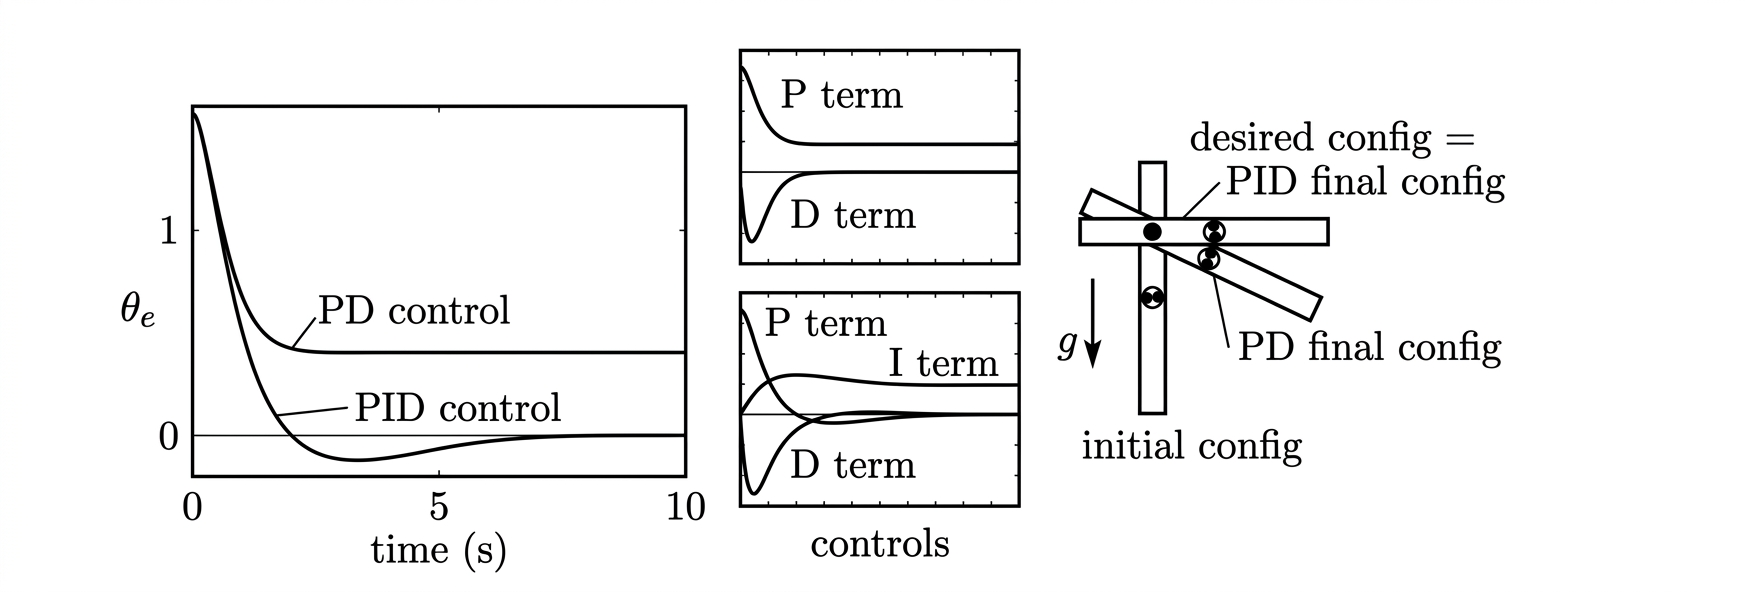
\includegraphics[width=0.8\linewidth]{img/pid.png}
\end{figure}

For attitude control, The error between the target orientation $q_{\text{target}}$ and the current body orientation $q_{\text{body}}$ is defined as \cref{eq:attitude}.

\begin{equation}\label{eq:attitude}
    \Delta q = q_{\text{target}} \cdot q_{\text{body}}^{-1}
\end{equation}

Using Unity's ToAngleAxis method, this relative rotation is converted into an angle $\phi$ and an axis $\mathbf{n}$. The error vector $\mathbf{e}$ is then $\mathbf{e} = \phi \cdot \mathbf{n}$.

The controller applies a PD loop (Proportional-Derivative) to generate corrective torque shown in \cref{eq:pdt}.

\begin{equation}\label{eq:pdt}
    \boldsymbol{\tau}_{\text{world}} = K_p \cdot \mathbf{e} + K_d \cdot \frac{\mathbf{e} - \mathbf{e}_{k-1}}{\Delta t}
\end{equation}

The world-space torque is transformed into the body frame ($R_{\text{wb}}$) for the physics simulation: $\boldsymbol{\tau}_{\text{body}} = R_{\text{wb}} \cdot \boldsymbol{\tau}_{\text{world}}$

The controller should be able to pilot the quadcopter in a closed-loop mission. The system employs a cascaded control scheme where the Outer Loop (Position) provides setpoints for the Inner Loop (Attitude/Velocity).

The Inner Loop features controllers that yield the required rolling and pitching moments $\tau_x$ and $\tau_y$ to regulate horizontal movement. The Inner Loop block requires the current quadcopter attitude as well as reference signals for roll and pitch to obtain its output \parencite{paredes2021quadcopter}; The Outer Loop, which features controllers that yield the required thrust differential and yawing moments as well as the desired reference signals.

During takeoff, the controller focuses exclusively on vertical error ($e_y$). The vertical force $force_Y$ is mapped to a normalized throttle value ($T$) shown in \cref{eq:mappingt}.

Following a path requires a look-ahead method. Given current position $\mathbf{p}$ and look-ahead target $\mathbf{t}$ on the path, the position error is defined as: $e_x = t_x - p_x,\quad e_y = t_y - p_y,\quad e_z = t_z - p_z$. 

The Outer Loop converts this error into a desired velocity in the world axis as shown in \cref{eq:outerLoop}.

\begin{equation}\label{eq:outerLoop}
    v_{x,\text{des}} = \text{PD}_X(e_x),\quad v_{z,\text{des}} = \text{PD}_Z(e_z)
\end{equation}

To translate these into drone-relative commands (Pitch/Roll), the world velocity is projected onto the drone's Heading Axis: (1) Forward Basis: $\hat{\mathbf{f}} = R_y(\psi)\,\hat{\mathbf{z}}_{\text{forward}}$; (2) Right Basis: $\hat{\mathbf{r}} = R_y(\psi)\,\hat{\mathbf{x}}_{\text{right}}$; The projections shown as \cref{eq:projection}. Where $e_{v,\parallel}$ is the longitudinal velocity error,  $e_{v,\perp}$ is the lateral velocity error.

\begin{equation}\label{eq:projection}
    v^{\parallel}_{\text{des}} = \mathbf{v}_{H,\text{des}}\cdot\hat{\mathbf{f}}, \quad v^{\perp}_{\text{des}} = \mathbf{v}_{H,\text{des}}\cdot\hat{\mathbf{r}}
\end{equation}

The Inner Loop then calculates the error between desired and actual velocity to produce stick inputs. Pitch (Right Vertical): Based on $e_{v,\parallel}$; Roll (Right Horizontal): Based on $e_{v,\perp}$.

The target yaw speed $\psi_{\text{target}} = \operatorname{atan2}(v_x,\,v_z)$, the yaw error is  $e_\psi = \text{DeltaAngle}(\psi, \psi_{\text{target}})$, so mapped to joystick movement is $u_{\text{yaw}} = \text{PID}_{\text{yaw}}(e_\psi)$. The other axis are the same methods.
\subsubsection{Design of a RL-Based HAC}

Alternatively, reinforcement learning (RL) can also be used in building an HAC agent with Unity's Machine Learning Agents (ML-Agents). ML-Agents allows developers to utilize games and simulations as training environments for intelligent agents. These agents can be trained using various paradigms, including reinforcement learning, imitation learning, and neuroevolution. Practical applications of trained agents encompass the control of non-player character (NPC) behavior in multi-agent or adversarial settings, automated game build testing, and the pre-release evaluation of game design decisions.

To facilitate training, a configuration file is typically required for the Python API, with Proximal Policy Optimization (PPO) serving as the predominant algorithm. The Python API interacts with the Unity environment via a communicator to execute the training process. Upon completion, the trained model is exported as an Open Neural Network Exchange (ONNX) file, which is subsequently used for agent inference and control. Furthermore, Unity provides a heuristic API for debugging and imitation learning (IL), enabling manual control over agents and the adjustment of training outcomes, as illustrated in \cref{fig:agent}.

\begin{figure}
    \caption{Simplified ML-Agents Scene Block Diagram}\label{fig:agent}
    \centering
\begin{tikzpicture}[
    font=\sffamily\bfseries,
    base/.style={rectangle, rounded corners=5pt, minimum width=2.2cm, minimum height=1cm, align=center, draw=white, line width=1pt, text=white},
    agent/.style={base, fill={rgb,255:red,119; green,184; blue,103}},
    behavior/.style={base, fill={rgb,255:red,98; green,155; blue,210}, minimum width=3cm},
    purple_box/.style={base, fill={rgb,255:red,146; green,106; blue,196}},
    orange_box/.style={base, fill={rgb,255:red,243; green,156; blue,87}},
    red_box/.style={base, fill={rgb,255:red,219; green,97; blue,94}},
    yellow_box/.style={base, fill={rgb,255:red,241; green,190; blue,47}},
    arrow/.style={<->, >=Stealth, thick, white},
    % 使用 * 并在连线时稍微偏移
    dash_arrow/.style={*-, dashed, thick, black} 
]

    % --- 内部节点 ---
    \node[behavior] (behA) {Behavior A};
    \node[agent, above left=1.5cm and -1.2cm of behA] (a1) {Agent\\A1};
    \node[agent, above right=1.5cm and -1.2cm of behA] (a2) {Agent\\A2};
    \node[orange_box, below=1cm of behA] (comm) {Communicator};

    \node[behavior, right=1cm of behA, minimum width=2.2cm] (behC) {Behavior C};
    \node[agent, at={(behC |- a1)}] (c1) {Agent\\C1};
    \node[purple_box, below=1cm of behC] (inf) {Inference};

    \node[behavior, right=1cm of behC, minimum width=2.2cm] (behD) {Behavior D};
    \node[agent, at={(behD |- a1)}] (d1) {Agent\\D1};
    \node[purple_box, below=1cm of behD] (heu) {Heuristic};

    % --- 外部节点 ---
    \node[red_box, below=2cm of comm] (pyAPI) {Python API};
    \node[yellow_box, right=1.2cm of pyAPI] (pyTrain) {Python Trainer};

    % --- 连线 ---
    \draw[arrow] (behA.north) -- ++(0,0.6) -| (a1.south);
    \draw[arrow] (behA.north) -- ++(0,0.6) -| (a2.south);
    \draw[arrow] (behA) -- (comm);
    \draw[arrow] (c1) -- (behC);
    \draw[arrow] (behC) -- (inf);
    \draw[arrow] (d1) -- (behD);
    \draw[arrow] (behD) -- (heu);
    
    % 虚线连线：起点从 comm.south 稍微往下移 1pt，确保圆点（*）不被框线切掉
    \draw[dash_arrow] ([yshift=-1pt]comm.south) -- (pyAPI.north);
    \draw[arrow, black] (pyAPI) -- (pyTrain);

    % --- 背景框 ---
    \begin{scope}[on background layer]
        % 增加 inner ysep=30pt 确保上下都有足够的留白
        \node[fill=gray, rounded corners=10pt, 
              fit=(a1) (a2) (c1) (d1) (comm) (inf) (heu), 
              inner xsep=15pt, inner ysep=30pt] (env) {};
        
        \node[anchor=north west, text=white, inner sep=10pt] at (env.north west) {Learning Environment};
    \end{scope}

\end{tikzpicture}
\end{figure}


For this research, each Drone Agent includes, (1) Agent Script, Handles OnActionReceived (processing joystick inputs), CollectObservations (monitoring states), and Heuristic (manual control for debugging); (2) Behavior Parameters: Defines the vector space for actions and observations. (3) Decision Requester: Controls the frequency of actions. By limiting the request rate, we can simulate more human-like reaction times, making the agent a better tutor for human pilots.

Proximal Policy Optimization (PPO) is an on-policy actor-critic algorithm that updates policies in small, clipped steps to ensure stability \parencite{openai2017ppo}. PPO is particularly effective for drones learning to navigate complex environments \parencite{yu2025depth}.

The optimization objective is defined as \cref{eq:ppo} shows.

\begin{equation}\label{eq:ppo}
L^{CLIP}(\theta) = \hat{\mathbb{E}}_t [ \min(r_t(\theta)\hat{A}_t, \text{clip}(r_t(\theta), 1-\epsilon, 1+\epsilon)\hat{A}_t) ]
\end{equation}

\begin{itemize}
    \item $\theta$ is the policy parameter
    \item $\hat{E}_t$ denotes the empirical expectation over timesteps
    \item $r_t$ is the ratio of the probability under the new and old policies, respectively
    \item $\hat{A}_t$ is the estimated advantage at time $t$
    \item $\epsilon$ is a hyperparameter, usually $0.1$ or $0.2$
\end{itemize}

Compared with a PID AI agent, a reinforcement learning-based AI agent does not require repeated testing to fine-tune parameters. Decisions are executed through a Decision Requester, which makes it easier to adjust the request frequency and pacing. However, as a black-box approach, it can be more difficult to achieve optimal performance or interpret and refine its behavior.


% Object: XR interactions



%--------------------------------------------%
\subsection{System Design Overview}

\subsubsection{Archetecture}

\subsubsection{Models}

%--------------------------------------------%
\subsection{Environment Construction}

%--------------------------------------------%
\subsection{Interaction and Control Design}





\section{Comparison of Current XR Development Platforms}

XR development is heavily dictated by the choice of game engine. Before initiating a project, it is critical to determine the target hardware and environmental requirements, as these factors define the development constraints.

Due to hardware availability, this paper focuses exclusively on development for the Meta Quest 3.

\subsubsection{Hardware Architectures: PC VR vs. Standalone}

For Head-Mounted Devices (HMDs) like the Meta Quest, two primary architectural configurations exist:

PC VR (Tethered): The headset acts as a peripheral. Assets are rendered on a high-end PC and streamed to the device via a wired (Link) or wireless (Air Link) connection. This allows developers to utilize the full power of engines like Unreal Engine, enabling high-fidelity features such as Lumen and Nanite. PC VR also supports specialized peripherals like haptic suits or omnidirectional treadmills, as seen in industry-standard titles like Half-Life: Alyx.

Standalone VR (All-in-One): Standalone headsets are self-contained systems with internal mobile chipsets. These provide high mobility but require significant optimization. High-end features must often be disabled or simplified to maintain performance. However, lightweight engines like Unity or Godot excel in this space, offering a balance between visual quality and mobile performance.

Rendevski et al. (2022) note that Standalone VR (SVR) applications offer significant advantages over PC VR. With proper optimization techniques, almost any PC VR scenario can be developed and deployed as SVR while still providing an acceptable user experience.

Differently, a recent survey from the Game Developers Conference (GDC) shows that among developers interested in creating VR/AR/MR games, the SteamVR platform (PC VR) slightly surpassed the Meta Quest / Horizon Store (68\% vs. 64\%) as their platform of interest. These were followed by PlayStation VR/VR2 (34\%) and Apple visionOS (15\%). However, when filtering for developers who have actually worked on VR/AR/MR games, a strong preference remains for the Meta Quest (72\%) over SteamVR (59\%).

\subsubsection{Passthrough (video see-through)}

Mixed reality (MR) headsets create immersive experiences designed to spatially integrate virtual content into the physical world. The newest headsets rely on passthrough video. While using passthrough, a person does not see light from the real world but instead relies on stereoscopic, color, high resolution, low latency, real-time video of the world, which is displayed on small screens inside a headset.(Bailenson et al., 2024)

Waldow et al. (2025) investigates Pass-Through Embodiment (PTE), The study found that PTE significantly enhances the user’s sense of presence and embodiment compared to using a customizable digital avatar. The ability to see one’s own body strengthens the feeling of being physically "present" in the VR environment without negatively affecting performance or causing sickness.

Leveraging passthrough on modern XR devices can help developers build highly engaging mixed-reality environments, which is particularly beneficial for applications like prototyping drone simulations.

\subsubsection{Software Standards}

To ensure cross-platform compatibility, developers rely on unified industry standards. Currently, there are two major public standards:

- OpenXR
- WebXR

\subsubsection{OpenXR}


OpenXR is the industry-standard API for XR applications. It is the interface between an application and an in-process or out-of-process “XR runtime system”. The runtime system handles functionality such as frame composition, peripheral management, and raw tracking information (Khronos OpenXR Working Group, 2024). Major game engines and the Meta Spatial SDK are built upon OpenXR to ensure hardware-agnostic development.

A primary bottleneck in XR development is the "deployment loop." Compiling a standalone APK and pushing it to a device can take 10–15 minutes per iteration.

- Link Mode: Developers often use the Oculus Link App to preview scenes in PC VR, though this requires constantly putting on and taking off the headset.

- Simulators: The Meta XR Simulator is increasingly becoming the preferred method for rapid iteration, allowing developers to simulate head and controller movements directly on their PC without needing physical hardware.

\subsubsection{WebXR}

The WebXR Device API provides the interfaces necessary to enable developers to build compelling, comfortable, and safe immersive applications on the web across a wide variety of hardware form factors (World Wide Web Consortium, 2022).

WebXR serves as a higher-level abstraction that runs in the browser, combining older specifications from WebVR and WebAR. The WebXR standard shares core features with and can be viewed as a subset of OpenXR.

While traditional game engines offer WebXR export support, there are fewer dedicated development stacks built exclusively for it. This section focuses specifically on engines that directly call the browser API.

For security reasons, WebXR APIs are restricted to HTTPS. Consequently, developers must use port-forwarding technologies during local development. Thanks to the efficiency of the web stack, a WebXR application typically only requires a few seconds to bundle. It is worth noting, however, that web rendering technology is currently transitioning from WebGL2 to WebGPU, which may introduce API changes in the WebXR ecosystem.


\subsubsection{Software Engine Comparison}

\begin{table}[h]
\centering
\begin{tabular}{l|l|l|l|l}
\hline
Feature & Unreal Engine (5.7) & Unity (6.0) & Godot (4.6) & Wonderland Engine \\
\hline
Primary Language & C++ / Blueprints & C\# & GDScript / C\# / C++ & JavaScript / TypeScript \\
Physics Engine & Chaos Physics & NVIDIA PhysX / DOTS & Jolt Physics (Integrated) & NVIDIA PhysX \\
Rendering Tech & Lumen (Dynamic GI) \& Nanite (Virtual Geometry) & URP / HDRP & Forward+ / Mobile & WebGL2 \\
Meta Support & Fork build & First-class Support & Community-driven (GDExtension) & No support \\
Machine Learning Support & Learning Agent & ML Agents & Godot RL Agents & No support \\
Editor Size (XR plugin included) & $\sim$50GB+ & $\sim$20GB & $<1$GB & 200MB \\
\hline
\end{tabular}
\caption{Comparison of game engines}
\end{table}

- Unreal Engine: UE is known for photorealistic rendering, UE provides unparalleled visual fidelity. Its Chaos Physics engine is highly regarded for complex simulations, making it the foundation for projects like Microsoft’s AirSim. However, UE has a high barrier to entry: the editor is massive, and utilizing Meta’s private APIs often requires compiling a custom engine branch from source.

- Unity: Unity remains the most popular choice for Meta Quest development due to its mature SDK support and C\# scripting. While it uses PhysX by default, its DOTS (Data-Oriented Technology Stack) provides high-performance physics for complex drone swarms. It offers the most streamlined "out-of-the-box" experience for Standalone VR.

- Godot: Godot has emerged as a powerful, lightweight alternative. It is highly compatible with modern AI coding assistants due to its Python-like GDScript. The integration of Jolt Physics as the default 3D engine has resolved previous performance hurdles for VR. However, its XR ecosystem is largely community-maintained. While excellent for prototyping, the lack of official Meta API support and the potential instability of third-party GDExtensions require careful dependency management for production-grade projects.

- Wonderland Engine: Wonderland Engine is a specialized WebXR engine built in C++ and compiled to WebAssembly.  By leveraging WebGL2, it achieves the performance necessary to render thousands of objects at native frame rates directly within a browser. . The development workflow relies on JavaScript and TypeScript, providing a highly familiar and accessible environment for traditional web developers. A unique advantage is the ability to edit scenes directly on the headset, enabling instant feedback without removing the device.




%--------------------------------------------%
\subsection{Learning System Design} % in discussion?

%--------------------------------------------%
\subsection{Data Collection Methods} % in discussion?

